\documentclass[12pt]{article}
\usepackage{ctex}
\usepackage{geometry}
\usepackage{graphicx}

\title{ResNet-18与Transformer}
\author{王逸群 19307110397}
\date{2022.5}

\geometry{a4paper,left=2.5cm,right=2.5cm,top=2.5cm,bottom=2.5cm}

\begin{document}
	
\maketitle

GitHub repo 链接:https://github.com/quniLcs/cv-final

网盘链接:

\section{数据集}

本项目使用CIFAR-100数据集,
其中包含60000张$32\times32$的彩色图片,
其中训练集50000张,测试集10000张,
被平均分为100类。

\section{网络结构}

\subsection{ResNet}

本项目使用的第一种网络结构是ResNet-18,
其中激活函数为ReLU,
最大的特征为残差连接。
后者包括两种单元结构如图\ref{fig:ResNetI}
和图\ref{fig:ResNetII}所示。

\begin{figure}[p]
	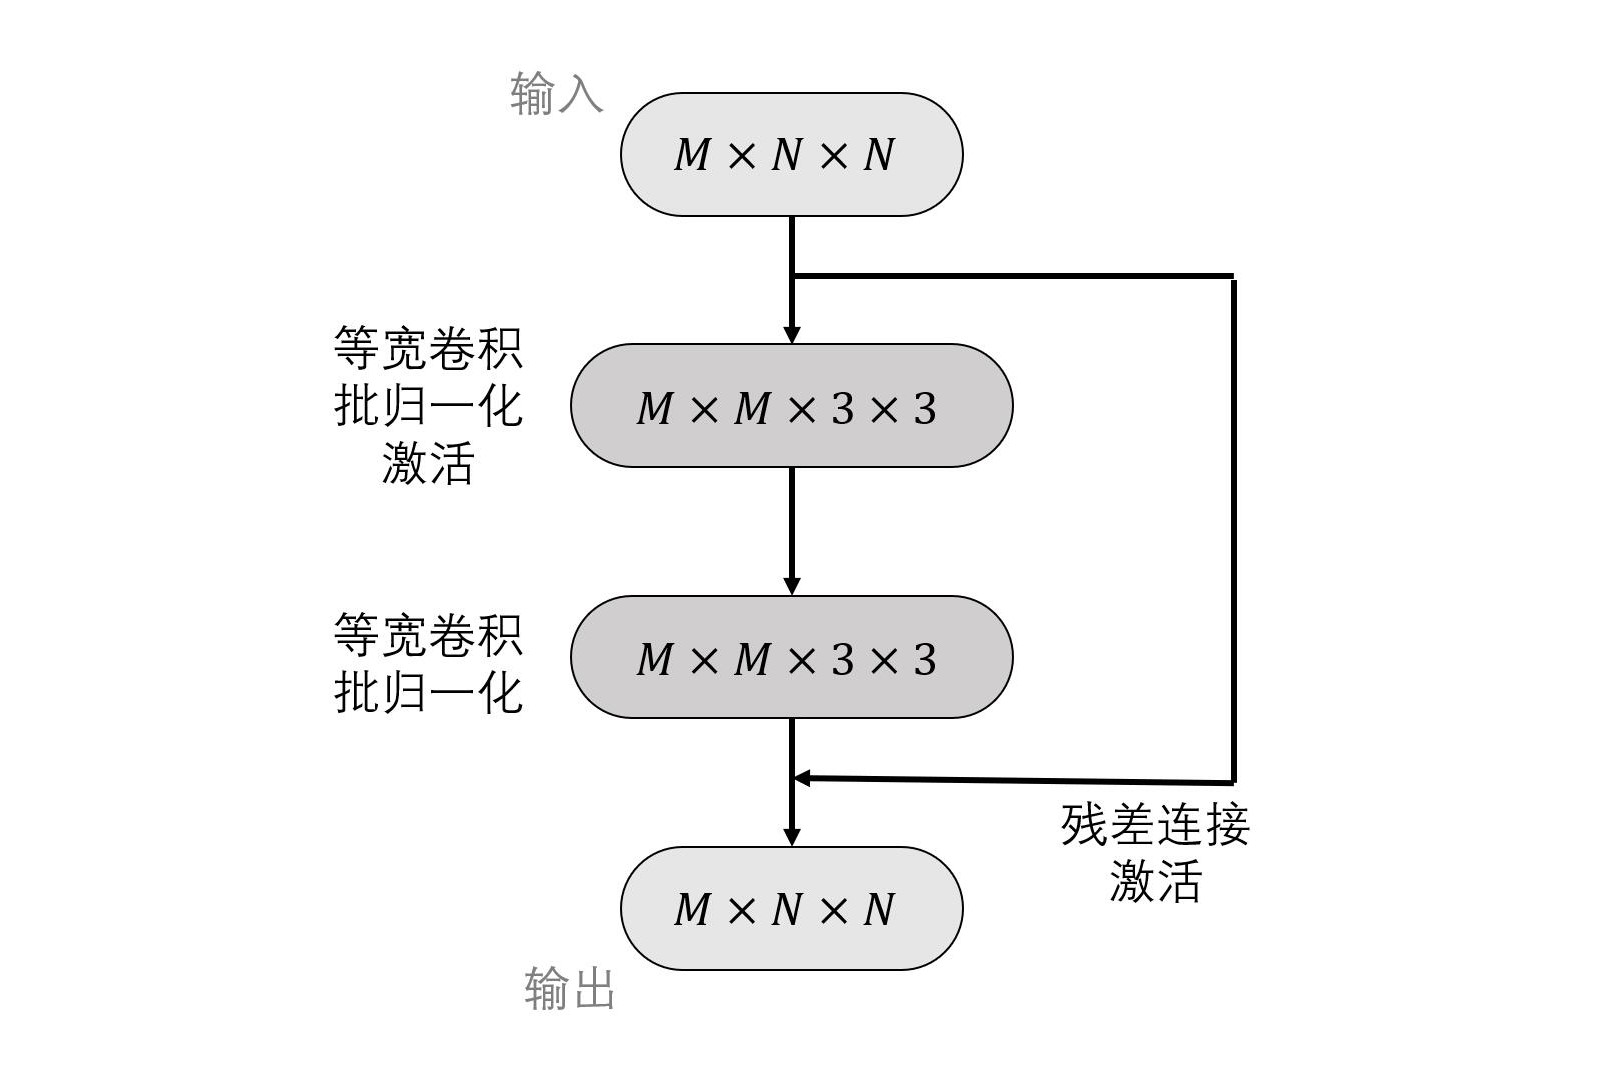
\includegraphics[width=\linewidth]{graph/ResNetI.jpg}
	\caption{残差连接第一种单元结构}
	\label{fig:ResNetI}
\end{figure}

\begin{figure}[p]
	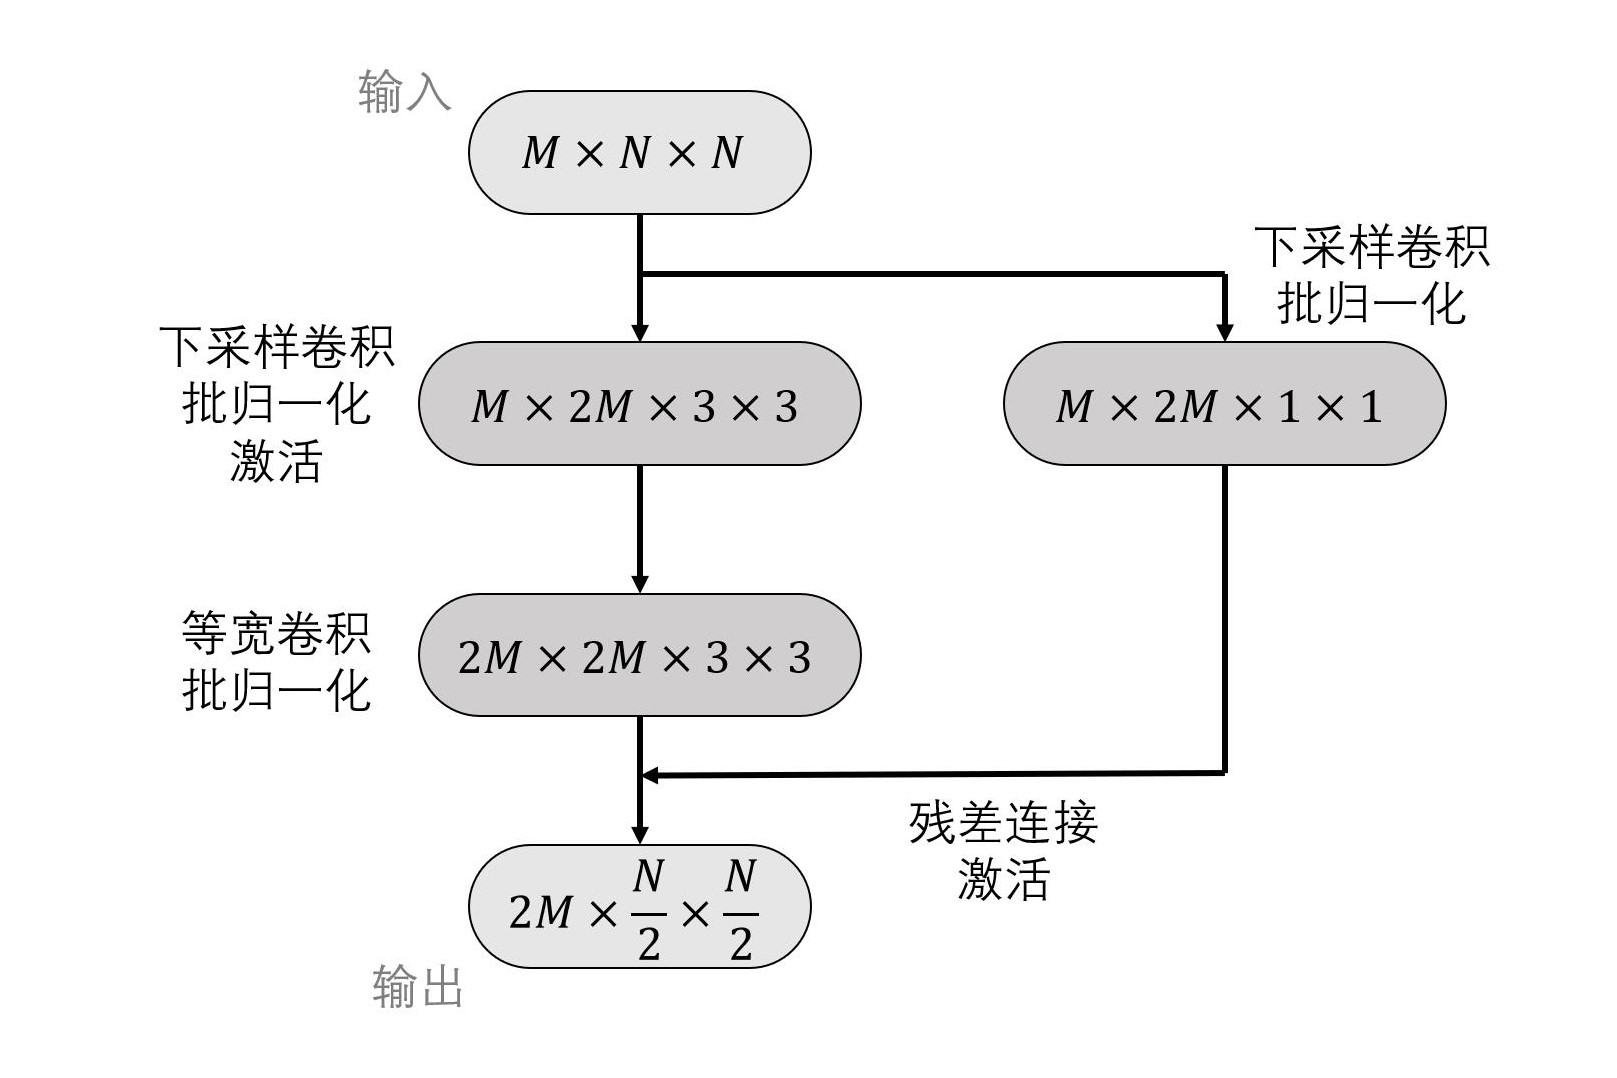
\includegraphics[width=\linewidth]{graph/ResNetII.jpg}
	\caption{残差连接第二种单元结构}
	\label{fig:ResNetII}
\end{figure}

对于输入的图像,
先进行步长为1的$3\times64\times3\times3$卷积操作,
并进行批归一化和激活,
维度变为$64\times32\times32$;
接着通过两次第一种单元结构,维度不变;
再通过第二种单元结构,维度变为$128\times16\times16$;
再通过第一种单元结构,维度不变;
再通过第二种单元结构,维度变为$256\times8\times8$;
再通过第一种单元结构,维度不变;
再通过第二种单元结构,维度变为$512\times4\times4$;
再通过第一种单元结构,维度不变;
最后通过全连接得到输出。

\subsection{Transformer}

\section{超参数设置}

数据增强:裁剪、水平翻转、CutOut;

参数初始化:MSRA;

学习率:由0.1开始每10个回合阶梯下降一个数量级;

优化器:带有0.9动量的随机梯度下降算法;

正则化参数:0.0005;

回合数:40;

批量大小:128;

每回合循环数:391;

总循环数:$ 40 \times 391 = 15640$;

损失函数:交叉熵损失函数;

评价指标:精确度。

\section{实验结果}
	
\end{document}